\documentclass[14pt,]{article}
\usepackage{lmodern}
\usepackage{amssymb,amsmath}
\usepackage{ifxetex,ifluatex}
\usepackage{fixltx2e} % provides \textsubscript
\ifnum 0\ifxetex 1\fi\ifluatex 1\fi=0 % if pdftex
  \usepackage[T1]{fontenc}
  \usepackage[utf8]{inputenc}
\else % if luatex or xelatex
  \ifxetex
    \usepackage{mathspec}
  \else
    \usepackage{fontspec}
  \fi
  \defaultfontfeatures{Ligatures=TeX,Scale=MatchLowercase}
    \setsansfont[]{GFS Neohellenic}
\fi
% use upquote if available, for straight quotes in verbatim environments
\IfFileExists{upquote.sty}{\usepackage{upquote}}{}
% use microtype if available
\IfFileExists{microtype.sty}{%
\usepackage{microtype}
\UseMicrotypeSet[protrusion]{basicmath} % disable protrusion for tt fonts
}{}
\usepackage[margin=1in]{geometry}
\usepackage{hyperref}
\hypersetup{unicode=true,
            pdftitle={Shall we move to more sophisticated methods to investigate subgroups in individual participant data meta-analysis?},
            pdfauthor={Michail Belias},
            pdfborder={0 0 0},
            breaklinks=true}
\urlstyle{same}  % don't use monospace font for urls
\usepackage{graphicx,grffile}
\makeatletter
\def\maxwidth{\ifdim\Gin@nat@width>\linewidth\linewidth\else\Gin@nat@width\fi}
\def\maxheight{\ifdim\Gin@nat@height>\textheight\textheight\else\Gin@nat@height\fi}
\makeatother
% Scale images if necessary, so that they will not overflow the page
% margins by default, and it is still possible to overwrite the defaults
% using explicit options in \includegraphics[width, height, ...]{}
\setkeys{Gin}{width=\maxwidth,height=\maxheight,keepaspectratio}
\IfFileExists{parskip.sty}{%
\usepackage{parskip}
}{% else
\setlength{\parindent}{0pt}
\setlength{\parskip}{6pt plus 2pt minus 1pt}
}
\setlength{\emergencystretch}{3em}  % prevent overfull lines
\providecommand{\tightlist}{%
  \setlength{\itemsep}{0pt}\setlength{\parskip}{0pt}}
\setcounter{secnumdepth}{0}
% Redefines (sub)paragraphs to behave more like sections
\ifx\paragraph\undefined\else
\let\oldparagraph\paragraph
\renewcommand{\paragraph}[1]{\oldparagraph{#1}\mbox{}}
\fi
\ifx\subparagraph\undefined\else
\let\oldsubparagraph\subparagraph
\renewcommand{\subparagraph}[1]{\oldsubparagraph{#1}\mbox{}}
\fi

%%% Use protect on footnotes to avoid problems with footnotes in titles
\let\rmarkdownfootnote\footnote%
\def\footnote{\protect\rmarkdownfootnote}

%%% Change title format to be more compact
\usepackage{titling}

% Create subtitle command for use in maketitle
\providecommand{\subtitle}[1]{
  \posttitle{
    \begin{center}\large#1\end{center}
    }
}

\setlength{\droptitle}{-2em}

  \title{Shall we move to more sophisticated methods to investigate subgroups in
individual participant data meta-analysis?}
    \pretitle{\vspace{\droptitle}\centering\huge}
  \posttitle{\par}
    \author{Michail Belias}
    \preauthor{\centering\large\emph}
  \postauthor{\par}
      \predate{\centering\large\emph}
  \postdate{\par}
    \date{03 June, 2019}

\usepackage{booktabs}
\usepackage{longtable}
\usepackage{array}
\usepackage{multirow}
\usepackage{wrapfig}
\usepackage{float}
\usepackage{colortbl}
\usepackage{pdflscape}
\usepackage{tabu}
\usepackage{threeparttable}
\usepackage{threeparttablex}
\usepackage[normalem]{ulem}
\usepackage{makecell}
\usepackage{xcolor}

\usepackage{bbm}
\usepackage{booktabs}
\usepackage{longtable}
\usepackage{array}
\usepackage{dsfont}
\usepackage{multirow}
\usepackage[table]{xcolor}
\usepackage{wrapfig}
\usepackage{float}
\usepackage{colortbl}
\usepackage{pdflscape}
\usepackage{tabu}
\usepackage{threeparttable}
\usepackage{threeparttablex}
\usepackage[normalem]{ulem}
\usepackage{makecell}
\newcommand{\blandscape}{\begin{landscape}}
\newcommand{\elandscape}{\end{landscape}}

\begin{document}
\maketitle

\hypertarget{abstract-116-out-of-200-words}{%
\section{Abstract (116 out of 200
words)}\label{abstract-116-out-of-200-words}}

\hypertarget{background}{%
\subsection{Background}\label{background}}

Individual participant data(IPD) meta-analysis(MA) is considered the
golden standard to investigate effect modification. Often treatment is
modified over continuous variables, which is a challenging task to
investigate and model their association with the outcome.

\hypertarget{objective}{%
\subsection{Objective}\label{objective}}

To overview recursive portioning (tree-based) and regression-based
approaches that detect and model effect-modification in meta-analysis of
individual participant data (IPD). We hereto consider one-stage
regression methods (linear, fractional polynomials and splines mixed
effects models), two-stage regression methods (meta-analysis of linear,
fractional polynomials models), meta-stepp(a sliding window approach)
and GLMM-trees, a recursive portioning method that takes also into
account the within trials clustering of the participants. Although,
regression-based methods can be used to confirm and to explore potential
effect modification, tree-based methods are suitable only for the later.

\hypertarget{study-design-and-setting}{%
\subsection{Study Design and Setting}\label{study-design-and-setting}}

We applied the approaches on two empirical data-sets. First, we
investigated the three-way effect modification of somatostatin by age
combined with gender on liver reduction in participants with polycystic
liver disease. Second, we investigated the three-way effect modification
of antibiotics by age and bilateral otitis on fever/ear-pain reduction
in children with acute otitis media.

\hypertarget{results}{%
\subsection{Results}\label{results}}

We show that GLMM-trees is a helpful exploratory tool, providing for
GLMM-trees, we found evidence of three-way interactions between
{[}\ldots{]}, {[}\ldots{]} and {[}\ldots{]}. One-stage regression found
evidence of effect modification by {[}\ldots{} {]}. Two-stage regression
found evidence of effect modification by {[}\ldots{]}. Unfortunately,
some two-stage approaches suffered from non-convergence, and lead to
omission of entire trials due to missing data . Different results w.r.t.
the presence of effect modifiers, the precision of their effects, and
the decision cut-points.

\hypertarget{conclusion}{%
\subsection{Conclusion}\label{conclusion}}

We conclude that the evaluation of subgroup effects due to effect
modification in IPD-MA requires careful consideration of modelling
assumptions, as effect modification may be distorted by unadjusted
non-linear associations and non-convergence . We therefore propose to
use flexible approaches such as GLMM-trees and one-stage regression
models with splines to explore and investigate effect modification in
IPD setting.

\newpage

\hypertarget{section}{%
\subparagraph{}\label{section}}

\hypertarget{introduction}{%
\section{1. Introduction}\label{introduction}}

Individual participant data meta-analysis (IPD-MA) is a type of
statistical analysis, where data are gathered from multiple studies are
combined and analysed. The capability to standardise subgroup
definitions and outcomes across studies, the increased power to
investigate other than linear associations, the increased validity and
reliability of the subgroups and the flexibility to search for subgroups
based on combinations of patient and/or disease characteristics are some
of the benefits of using IPD of multiple trials rather than traditional
(aggregate) meta-analysis {[}1--3{]}. A vivid field of research towards
personalised healthcare is the investigation of effect modification. For
this, IPD-MA is considered the gold standard as single trials rarely
have sufficient power to properly detect effect modification. Effect
modification may be present in both categorical and/or continuous
covariates. For instance, differences in the treatment effect may be
present between smokers and non-smokers, or across the age of the
patients. If subgroups have been predefined, hypothesis testing may be
performed using traditional regression-based methods. For single trials,
this typically involves the estimation of (linear) interaction terms
between treatment and the modifier of interest. In an IPD-MA, these
interaction effects may be estimated either separately within studies
and subsequently be pooled across studies (two-stage IPDMA), or directly
across all studies (one-stage IPDMA. However, effect modification across
a continuous variable is more challenging, since we may need to evaluate
effect modification and at the same time want to define a threshold from
which point the treatment effect is relevantly different. This way the
continuous variable is categorised into subgroups, where the clinician
can make decision whether to treat or not treat. Reversely, the same
notion is used to analyse data. Categorization is a common technique to
investigate effect modification, by splitting the continuous covariate
into subgroups. Nevertheless, these subgroups should always be created
based on good prior knowledge from literature. If so, this approach can
be meaningful. In all other cases, categorization has been criticised
for misspecification, loss of information and power, inflation of the
type I error rate and even biased results {[}4--8{]}. Another common
practice is using the continuous variable as it is, and assume linearity
on the linear predictor scale . This approach may also lead to
deterioration of power, misspecification, and even spurious results if
the true relationship is not linear {[}9{]}. Both categorisation and
false functional form assumptions are prone to significant ecological
bias. For instance, if the functional form of mortality and age is
exponential and some trials have old participants while other young,
both approaches can lead to biased pooled results. Ideally, when
continuous covariates are included, we would like to account for their
functional form, while simultaneously making inferences over the
presence of the effect modification and avoiding ecological.
Furthermore, although the association between the outcome and the
continuous effect modifier is highly informative, clinical decisions are
based on subgroups of participants the differ in treatment response.
Finally, subgroups generated from continuous variables are defined by
the cut-points were the treatment effect is considered to change. These
cut-points may be based on the treatment effect function {[}10{]},
i.e.~the difference between the two treatments over the range of the
covariable or the treatment-effect modifier interaction terms {[}11{]}.
For this, various approaches to account for non-linear associations have
been developed, such as splines and fractional polynomials (FP)
{[}12{]}.

\par

For IPD-MA, regression-based approaches such as linear models, piecewise
polynomials, FPs and smoothing splines may be performed either in one or
two stages. In a two-stage approach, each trial is first modelled
separately using an appropriate statistical model. Subsequently, we pool
either the extracted coefficients if shared across the trials or their
fitted functions, using standard meta-analytical tools. In contrast, in
one-stage IPD-MA the IPD from all trials are analysed simultaneously
whilst accounting for the clustering of participants within studies .
Hereto, we model interactions between treatment and patient-level
variables while accounting also for the shape of the associations with
the outcome. Recent recommendations suggest mean-centring the potential
effect modifiers per trial in order to account for potential ecological
bias due to unadjusted confounding. In such a one-stage model,
within-trial clustering can be accounted for using either a fixed effect
(common intercept/slope), fixed effects (stratified intercept/slope), or
random effects {[}13{]}. Other methods to explore effect modification
are plot- and tree-based methods such as the generalised linear
mixed-effects model tree (GLMM-tree) method {[}14{]} or meta-stepp, a
moving average (sliding window) method.

\par

Although there is a large variety of methods to explore effect
modification for continuous covariates, little guidance exists on their
use. We aim to describe and illustrate the aforementioned methods by
applying them on two empirical examples, while discussing their
(potential) advantages and limitations.

\hypertarget{empirical-examples}{%
\section{2. Empirical examples}\label{empirical-examples}}

\par

WWe use 2 IPD-sets to illustrate aforementioned methods. The first
empirical example {[}15{]} considers an IPD-MA where the effect of
antibiotics in acute otitis media was investigated in children. Rovers
et al.~collected IPD from 6 randomised clinical trials with a total of
1643 children, aged from 0-12 years old. The primary outcome was fever
and/or ear-pain after 3-7 days (yes/no). They concluded that antibiotics
were more beneficial in younger children (less than 2 years old) with
bilateral acute otitis media. Bilateral acute otitis media (yes/no),
age, otorrhea were investigated also separately for potential effect
modification and only bilateral acute otitis media showed a significant
result. The second empirical example {[}16{]} considers an IPD-MA to
investigate the effect of Somatostatin on liver volume reduction. Gevers
et al.~collected IPD from 3 randomised placebo-controlled trials with a
total of 107 participants. In this example, the outcome was continuous
(liver volume reduction), and age, sex, baseline liver volume, and
diagnosis of either autosomal dominant polycystic liver or kidney
disease were investigated for effect modification . They concluded that
use of Somatostatin was more beneficial for younger (\textless47) female
patients. One of the 3 trials had a cross-over design, therefore
participants were treated both with the active and the control treatment
in different time periods. In order to use these data for our
illustrative purposes, we removed the cross-over design and used all
patients only once, by selecting half of the patients from the active
period and the other half (sex and age-matched) from the control period.
Therefore, differences between our results and those reported in the
original article may occur.

\begingroup\fontsize{8}{10}\selectfont

\begin{longtabu} to \linewidth {>{\raggedright}X>{\raggedright}X>{\raggedright}X>{\raggedright}X>{\raggedright}X>{\raggedright}X>{\raggedright}X}
\caption{\label{tab:unnamed-chunk-1}Baseline Characteristics (Gevers et al.)}\\
\toprule
\multicolumn{1}{c}{\textbf{ }} & \multicolumn{2}{c}{\textbf{van Keimpema et al}} & \multicolumn{2}{c}{\textbf{Hogan et al}} & \multicolumn{2}{c}{\textbf{Caroli et al}} \\
\cmidrule(l{3pt}r{3pt}){2-3} \cmidrule(l{3pt}r{3pt}){4-5} \cmidrule(l{3pt}r{3pt}){6-7}
\textbf{ } & \textbf{Placebo} & \textbf{Somatostatin} & \textbf{Placebo} & \textbf{Somatostatin} & \textbf{Placebo} & \textbf{Somatostatin}\\
\midrule
\rowcolor{gray!6}  Number of participants & 27 & 27 & 14 & 28 & 6 & 6\\
Age, median [range] & 48 [36,68] & 49 [32,65] & 49 [38,65] & 47 [34,69] & 39 [29,53] & 40 [30,59]\\
\rowcolor{gray!6}  Female & 23 (85\%) & 24 (89\%) & 13 (93\%) & 23 (82\%) & 2 (33\%) & 1 (17\%)\\
Male & 4 (15\%) & 3 (11\%) & 1 (7\%) & 5 (18\%) & 4 (67\%) & 5 (83\%)\\
\rowcolor{gray!6}  Log-scaled Liver volume difference, median [range] & 0.011 [-0.038,0.079] & -0.018 [-0.19,0.043] & -0.006 [-0.109,0.166] & -0.034 [-0.172,0.092] & -0.006 [-0.096,0.158] & -0.05 [-0.09,0.031]\\
\bottomrule
\end{longtabu}
\endgroup{}

\begin{landscape}\begingroup\fontsize{8}{10}\selectfont

\begin{longtabu} to \linewidth {>{\raggedright}X>{\raggedright}X>{\raggedright}X>{\raggedright}X>{\raggedright}X>{\raggedright}X>{\raggedright}X>{\raggedright}X>{\raggedright}X>{\raggedright}X>{\raggedright}X>{\raggedright}X>{\raggedright}X}
\caption{\label{tab:unnamed-chunk-1}Baseline Characteristics (Rovers et al.)}\\
\toprule
\multicolumn{1}{c}{\textbf{ }} & \multicolumn{2}{c}{\textbf{Damoiseaux}} & \multicolumn{2}{c}{\textbf{Burke}} & \multicolumn{2}{c}{\textbf{Appelman}} & \multicolumn{2}{c}{\textbf{Little}} & \multicolumn{2}{c}{\textbf{Saux}} & \multicolumn{2}{c}{\textbf{McCormick}} \\
\cmidrule(l{3pt}r{3pt}){2-3} \cmidrule(l{3pt}r{3pt}){4-5} \cmidrule(l{3pt}r{3pt}){6-7} \cmidrule(l{3pt}r{3pt}){8-9} \cmidrule(l{3pt}r{3pt}){10-11} \cmidrule(l{3pt}r{3pt}){12-13}
\textbf{ } & \textbf{Placebo} & \textbf{Antibiotics} & \textbf{Placebo} & \textbf{Antibiotics} & \textbf{Placebo} & \textbf{Antibiotics} & \textbf{Placebo} & \textbf{Antibiotics} & \textbf{Placebo} & \textbf{Antibiotics} & \textbf{Placebo} & \textbf{Antibiotics}\\
\midrule
\rowcolor{gray!6}  Number of participants & 123 & 117 & 118 & 114 & 54 & 67 & 164 & 151 & 254 & 258 & 111 & 112\\
Age, median [range] & 1 [1,2] & 1 [0,2] & 5 [3,9] & 5 [3,9] & 4.16 [1.07,10.22] & 3.83 [0.65,10.19] & 4.74 [0,10.87] & 5.03 [0.48,11.1] & 2.71 [0.55,5.97] & 2.86 [0.5,6.01] & 1.82 [0.51,12.66] & 1.46 [0.5,12.65]\\
\rowcolor{gray!6}  Males (\%) & 66 (54\%) & 64 (55\%) & 50 (42\%) & 59 (52\%) & 25 (46\%) & 31 (46\%) & 81 (49\%) & 74 (49\%) & 131 (52\%) & 129 (50\%) & 58 (52\%) & 54 (48\%)\\
Bilateral AOM (\%) & 76 (62\%) & 75 (64\%) & 16 (14\%) & 16 (14\%) & 6 (11\%) & 14 (21\%) & NA (NA\%) & NA (NA\%) & 74 (29\%) & 79 (31\%) & 48 (43\%) & 52 (46\%)\\
\rowcolor{gray!6}  Otorrhoea (\%) & 19 (15\%) & 16 (14\%) & NA (NA\%) & NA (NA\%) & NA (NA\%) & NA (NA\%) & 46 (28\%) & 35 (23\%) & NA (NA\%) & NA (NA\%) & NA (NA\%) & NA (NA\%)\\
\bottomrule
\end{longtabu}
\endgroup{}
\end{landscape}

\hypertarget{methods}{%
\section{3. Methods}\label{methods}}

\hypertarget{notation}{%
\subsection{3.1 Notation}\label{notation}}

As described in section 2, both empirical example datasets are composed
of multiple randomised trials. We will adopt the following notation
throughout our manuscript:

\begin{itemize}
\tightlist
\item
  The trials as j = 1,2, \ldots,\(n_j\),
\item
  Trial participants as i = 1,2, \ldots,\(n_i\),
\item
  The per trial mean of age as \(\bar{Age_j}\)
\item
  The per trial centred age as \(X_{ij}\) = \(\bar{Age_j} - Age_{ij}\)
\item
  Cut-point (knot) as \(\kappa\)
\item
  The degree of a fractional polynomial as m
\item
  The degree of a polynomial as p
\end{itemize}

\hypertarget{recursive-partitioning-tree-based-methods}{%
\subsection{3.2. Recursive-partitioning (tree-based)
methods}\label{recursive-partitioning-tree-based-methods}}

Recursive partitioning can be a first step to explore the underlying
structure of the data, such as whether there are outcome differences
across the levels of a continuous or categorical variable. It is a
statistical method typically used in multivariable analysis {[}17{]}. A
decision tree is generated by dichotomising the variable by cut-points
creating subgroups, thus creating subgroups where the treatment effect
is altered. Recursive partitioning techniques can handle non-linear
associations as they make no functional form assumption a-priori.\\

\par

Splitting the data-set into subgroups is a sensitive process. Therefore,
it is highly important to account for within trial clustering of the
participants. The Generalised linear mixed model (GLMM) tree approach is
a state-of-the-art technique using a model-based recursive partitioning
{[}18,19{]} algorithm. It was proposed by Fokkema et al.~{[}20{]} to
detect treatment-effect modifier interactions in the presence of
clustered data, as is the case in IPD-MA. Since this approach is
exploratory, we can play with the significance level \(\alpha\) for the
splitting criterion, to be more or less liberal. Furthermore, we can use
GLMM-trees to detect the possibly relevant variables, their crude
cut-points and their underlying subgroups. If GLMM-tree results in
subgroups, we can evaluate the corresponding variable using a more
sophisticated approach. For example, if we identify age and gender as
subgrouping variables using the GLMM-tree, we can use a regression
technique to model this relationship. The GLMM tree algorithm (1) starts
by fitting a regression model with interaction terms (treatment x
subgroup variables) included (2) statistically tests the interaction
terms using a user-defined α, i.e.~whether treatment is modified with
respect to the subgroup variables, then (3) if test indicates
modification, splits the dataset in order to create 2 subgroups with the
largest difference in treatment effect. This procedure is (4) repeated
in each of the resulting subgroups, until a user-defined convergence is
achieved.

\hypertarget{regression-based-approaches}{%
\subsection{3.3 Regression based
approaches}\label{regression-based-approaches}}

\par

In regression-based approaches it is important to specify an appropriate
functional form for the association between the effect modifier and the
outcome. If the functional form is known a priori (e.g.~linear,
log-linear), modelling is fairly straightforward. However, if the
functional form is not properly be predefined, splines and/or fractional
polynomials may be used to evaluate the functional form of the
association.

\par

When using segmented functions, another concern is the selection and
placing of the cut-points (knots), which are used to model changes in
the shape of the association. The location and number of knots could be
either predefined or estimated. In first case, we split the variable in
these knots and fit an appropriate polynomial regression within. In the
later, we may either use cross-validation or penalised maximum
likelihood approaches .

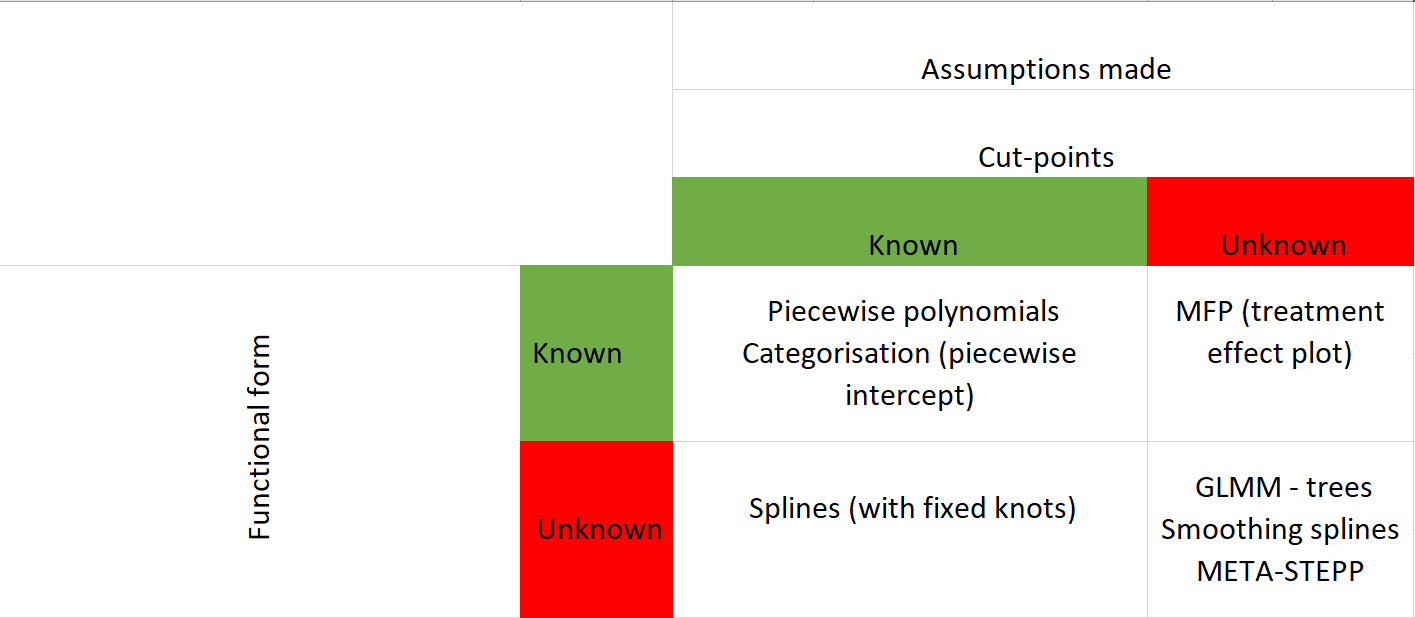
\includegraphics[width=0.8\linewidth,height=0.8\textheight]{Figs/Assumption}

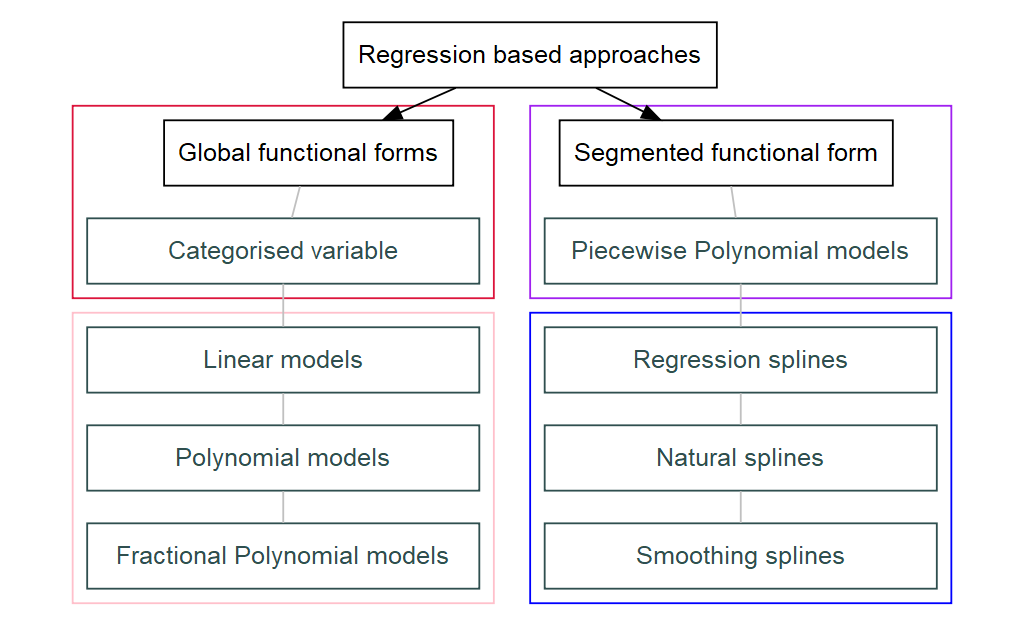
\includegraphics[width=0.8\linewidth,height=0.8\textheight]{Figs/TypesOfMethods}

Finally, for any regression-based approach, the presence of within-trial
clustering should be accounted for {[}21{]}. Below, we describe how this
can be done in an IPD-MA.

\begin{table}[t]

\caption{\label{tab:unnamed-chunk-4}Characteristics of the methods}
\centering
\resizebox{\linewidth}{!}{
\begin{tabular}{>{\bfseries\raggedright\arraybackslash}p{10em}>{\raggedright\arraybackslash}p{10em}>{\raggedright\arraybackslash}p{6em}>{\raggedright\arraybackslash}p{10em}llll}
\toprule
Statistical methods & Type of second stage pooling & Fit near the edges & Cut-points & Degrees of freedom spent & Difficulty & Converged & Trials excluded\\
\midrule
\rowcolor{gray!6}   & Coefficient  or fitted functions pooling &  &  & [Liver data, AOM data] &  &  & [Liver data, AOM data]\\
 &  &  &  &  &  &  \vphantom{4} & \\
\rowcolor{gray!6}   &  &  &  &  &  &  \vphantom{3} & \\
Global methods\rowcolor{gray!6}   &  &  &  &  &  &  \vphantom{2} & \\
\rowcolor{gray!6}  Fractional Polynomials (FP) & Both & medium & None & [21 , 32] & Easy & Only overall FP method & [0 , 3]\\
\addlinespace
Generalised linear models & Both & Bad & None & [21,] & Easy &  & \\
\rowcolor{gray!6}  Generalised linear mixed effects models & NA & Bad & None &  & Moderate &  & \\
Mixed effects fractional polynomials &  &  &  &  & Moderate &  & \\
 &  &  &  &  &  &  \vphantom{1} & \\
Segmented methods\rowcolor{gray!6}   &  &  &  &  &  &  & \\
\addlinespace
\rowcolor{gray!6}  Piecewise polynomials & Both & Good & Predifined &  & Difficult &  & \\
Splines & only fitted functions & Good & Predifined & [8.6, 13.79] & Moderate &  & \\
\rowcolor{gray!6}  Natural splines & only fitted functions & Special & Predifined &  & Moderate &  & \\
Smoothing splines & only fitted functions & Best & Not necessary &  & Moderate &  & \\
\rowcolor{gray!6}  Generalised additive models & NA & Best & Not necessary & [8.6, 13.79] & Difficult &  & \\
\addlinespace
 &  &  &  &  &  &  & \\
 &  &  &  &  &  &  & \\
 &  &  &  & Abbreviations &  &  & \\
\rowcolor{gray!6}   &  &  &  & l: the levels of the treatment &  &  & \\
 &  &  &  & k: \# of the cut-points &  &  & \\
\addlinespace
\rowcolor{gray!6}   &  &  &  & j: \# of trials &  &  & \\
 &  &  &  & i: \# of participants per trial &  &  & \\
\rowcolor{gray!6}   &  &  &  & m: order of the FP &  &  & \\
 &  &  &  & Coef : Coefficients with random effects &  &  & \\
\bottomrule
\end{tabular}}
\end{table}

\hypertarget{two-stage-approaches}{%
\subsubsection{3.3.1. Two-stage approaches}\label{two-stage-approaches}}

In two-stage approaches a statistical model of choice is directly fitted
per trial. The statistical model per trial j is as follows:

\[g(Y_{ij}) = \hat f_{1j}(X)  + \hat f_{2j}(X) \times Treatment\]

\begin{flushright} [1] \end{flushright}

Subsequently, we can either pool the coefficients or the fitted
functions using typical meta-analytical tools.

\hypertarget{first-stage-per-trial-modelling}{%
\paragraph{3.3.1.1 First stage: Per-trial
modelling}\label{first-stage-per-trial-modelling}}

The functions \(\hat f_{1j}, \hat f_{2j}\) are providing the functional
shape of the outcome-effect modifier association per trial j for the
treated and the control group respectively. Depending on the a priori
knowledge of the association's functional form and the cut-points where
the effect is altered, we may either fit a generalised additive model
with splines included, a fractional polynomial model or a polynomial
model (including linear shapes and categorised variable). The approaches
mentioned above, besides FPs, can be also performed using the continuous
variable split in predefined cut-points, also called knots.

\emph{Unknown functional form and known knots }

Splines are a generalisation of piecewise polynomials and can offer
great flexibility to explore the shape of the outcome-effect modifier
association. Regression splines of \textbf{p} degree should be
continuous, have \textbf{p-1} continuous derivatives and the \(p^{th}\)
derivative should constant across the knots. They are quite similar to
piecewise polynomials, with the difference that they are continuous
across the knots. A natural spline has an extra assumption that the
second derivative of the function over the edges \(k_0, k_{\kappa}\) is
0. This is a something that should be considered when the goal of our
research is to forecast future outcomes, as for instance in longitudinal
or time series studies. When using splines, the real underlying shape is
not known or we don't want to assume it is known, therefore, we explore
it. However, information over the position of the knots and their number
may be also unknown. Thus, we can introduce even more flexibility into
our model by fitting smoothing splines. Smoothing splines by-pass the
problem of knot selection by shrinking the coefficients to their basis
expansion, which is a piecewise polynomial. In order to do so, they
minimise the penalised least squares criterion or equivalently the
maximum likelihood criterion with an extra parameter representing the
wingliness of the line, \(MLE + \lambda\int_0^1[f^{''}(x)]^2 dx\)
equivalently \(|| y - X\beta ||^2 + \lambda\int_0^1[f^{''}(x)]^2 dx\) or
in algebraic form \(|| y - X\beta ||^2 + \lambda\beta^TS\beta\).

\emph{Unknown functional form and known \(\kappa = 0\) knots (global
function)}

Fractional polynomials {[}22{]} are an extension of polynomials, that
also include negative powers. FPs provide a global functional form. FPs
model the effect of a covariate X as
\(f(x;\beta) = \sum_{k=1}^{k=m} \beta_{k} \times X^{p_{k}}\), where m is
the degree of the fractional polynomial and the power is derived from a
fixed set of powers \(p_k \in S :\) \{-2,-1,-0.5, 0=(log),0.5,1,2\}. The
Fractional selection procedure FSP algorithm (FSP) has been proposed
{[}23{]} to explore the best fitting fractional polynomial. The
fractional polynomials of a common degree \textbf{m} are tested using
the deviance difference criterion, whilst fractional polynomials of
different degree are compared using a \(\chi^2\) test. When multiple
data-sets are present Sauerbrei and Royston {[}12{]}, have proposed 3
methods to evaluate the general functional form.

\begin{itemize}
\tightlist
\item
  Overall FP, where the FSP is applied in the pooled data, in order to
  find the best FP (stratified by data-set).
\item
  Study-wise FP2, the best FP2 is selected for each study
\item
  Study wise selected FP, where the best fitting FP is extracted per
  study
\end{itemize}

\emph{Known functional form and known \(\kappa \geq 1\) knots and known
position of the knots (segmented functions)}

\begin{itemize}
\tightlist
\item
  Piecewise-polynomials with \(\kappa\) knots
  \[f_1 = \sum_{k =1}^{ k= \kappa}f_{1\kappa}(X_{x_{k-1} \leq X < x_{k-1}} ) f_2 =  \sum_{k =1}^{k= \kappa}f_{2\kappa}(X_{x_{k-1} \leq X < x_{k-1}} )\]
  Piecewise-polynomials mostly used are piecewise constant, linear,
  quadratic and cubic.
\end{itemize}

\emph{Known functional form and known \(\kappa = 0\) knots (global
functions)}

\begin{itemize}
\tightlist
\item
  Global-polynomials:
\end{itemize}

\[f_1 =  \sum_{\pi=1}^{\pi=p} \beta_{1\pi} \times X^{\pi}\]
\[ f_2 = \sum_{\pi=1}^{\pi=p} \beta_{2\pi} \times X^{\pi}\] - Global
polynomials typically are limited to either linear, Quadratic or Cubic,
but can go to higher degrees.

\hypertarget{second-stage-combination-of-the-first-stage-results}{%
\paragraph{3.3.1.2 Second-stage combination of the first stage
results}\label{second-stage-combination-of-the-first-stage-results}}

As a second-stage in the two-stage IPD-MA, we either pool the estimates
or the fitted functions \(\hat f_{1j}(X)\), \(\hat f_{2j}(X)\) extracted
from the first stage. The simplest approach is to pool the extracted
trial \(\beta_{kj}\) into one \(b_k\), using a multi-variate
meta-analysis, whilst assuming a common effect or random effects. When
using random effects approach, a variety of methods is available to
estimate the pooled coefficients, such as maximum likelihood, restricted
maximum likelihood, method of moments or variance components. We
preferred the restricted maximum likelihood, in order to be consistent
with one-stage approaches. This approach only works when common powers
are present across studies. Therefore, it is applicable in piecewise,
global polynomials, and fractional polynomials fitted using the overall
FP procedure.

Another suggested pooling method is to pool the fitted functions. For
each x in the data (pointwise) we calculate per study the fitted
function \(\hat{g_j}(x; \beta_j)\) and its standard error from
\(SE_j(x)\). This \(\hat{g_j}(x; \beta_j)\) is the per trial predicted
line or equivalently the mean expected outcome for given x
E(g(x)\textbar X=x) and the \(S_j(x)\) is the confidence intervals of
the predicted line. Afterwards, for each x in the data (pointwise), we
calculate the pooled estimate \(\hat{g}(x)\) and its SE(x), using either
common or random-effects meta-analysis {[}25{]}.

\hypertarget{one-stage-approaches}{%
\subsubsection{3.3.2. One-stage approaches}\label{one-stage-approaches}}

\hypertarget{generalised-additive-mixed-effects-models}{%
\paragraph{3.3.2.1 Generalised additive mixed effects
models}\label{generalised-additive-mixed-effects-models}}

Generalised additive models are a form of penalised generalised linear
models. One type of penalization is identical to the random effects'
technique introduced by McCullagh et al.~{[}26{]} in the generalised
mixed effects models. There we can estimate a separate functional form
per trial, given the fixed effects parameters.

\hypertarget{multilevel-fractional-polynomials}{%
\paragraph{3.3.2.2 Multilevel Fractional
polynomials}\label{multilevel-fractional-polynomials}}

Fractional polynomials may be used using a one stage approach {[}27{]}.
In this case, we use the same set of powers as in the FSP method.
Furthermore, we fit a mixed effect model of our choice, with either
stratified, fixed or random effects. For model selection we can use the
model with the lowest deviance or the Akaike Information Criterion (AIC)
{[}29{]}, or Bayesian Information Criterion (BIC) {[}30{]}.

Therefore, the statistical model applied is:

\(g(Y_{ij}) = FP_{1j}(X) + FP_{2j}(X) \times Treatment\)

\hypertarget{centred-one-stage-ipd-ma}{%
\paragraph{3.3.2.3 Centred One-stage
IPD-MA}\label{centred-one-stage-ipd-ma}}

We follow recent recommendations {[}31{]} and centre per trial the
effect modifier. This way we can separate the within and across trial
information of the effect modification. As in the two stage methods we
can fit piecewise and global polynomials, but using a mixed-effect model
to account for within trials clustering. Therefore, assuming that
\(X_{ij} = Age_{ij} - \bar Age_j\), the statistical model will be:

\(g(Y_{ij}) = \hat f_{1j}(X) + \hat f_{2j}(X) \times Treatment\)

The \(\hat f_{1j}\) and \(\hat f_{2j}\) can be either piecewise
polynomials, global polynomials or splines as described in section
\emph{3.3.1.1}.

For the \(\beta_{1kpj}\) and \(\beta_{2kpj}\) we can assume, either
fixed (common) effect, fixed effect\emph{s} (stratified betas), or
random effects. If we choose the fixed effect approach a common beta is
assumed, in the stratified approach j betas will be generated which
correspond to the per trial beta, while in the random effects we assume
that the per trial coefficients are driven from a common Normal
distribution N(\(b, \sigma^2\)).

\newpage

\hypertarget{section-1}{%
\subparagraph{}\label{section-1}}

\hypertarget{results-1}{%
\section{Results}\label{results-1}}

We will illustrate the results of the aforementioned approaches
beginning with the more exploratory to the more confirmatory methods.
Therefore, we will start with the tree-based approach and smoothing
splines, as we believe that these should be the first exploratory steps.
Subsequently, we will show the results of FPs and we end with
generalised linear models. We will start with the liver disease data-set
and then show the results of the acute otitis media data-set.

\hypertarget{regression-based-approaches-1}{%
\subsection{Regression-based
approaches}\label{regression-based-approaches-1}}

We will show the results for each approach, first when performing a
two-stage method and then when using a one-stage method. The liver
disease data set contained trials with limited number of participants,
see table 1. For instance, Caroli et.al had only 1 female participant in
the somatostatin group. On the other hand, Keimpema et al.~and Hogan et
al.~had limited participation of men. Therefore, the liver data set was
impossible to be analysed using two-stage approaches, for the three-way
interaction we observed above. We present only the acute otitis media
approach. Before starting applying regression-based techniques to model
or identify interactions, we suggest to plot the data using a locally
estimated scatterplot smoothing (loess) approach, in order to have a
first touch with the variables and how they are associated. We will show
the results for each approach, first when performing a two-stage and
then when using a one-stage method. The liver disease data set contained
trials with limited number of participants, see table 1. For instance,
Caroli et.al had only 1 female participant in the somatostatin group. On
the other hand, Keimpema et al.~and Hogan et al.~had limited
participation of men. Therefore, the liver data set was impossible to be
analysed using two-stage approaches, for the three-way interaction we
observed above. We present only the acute otitis media approach.

Before starting applying regression-based techniques to model or
identify interactions, we suggest to plot the data using a locally
estimated scatterplot smoothing (loess) approach, in order to have a
first touch with the variables and how they are associated.

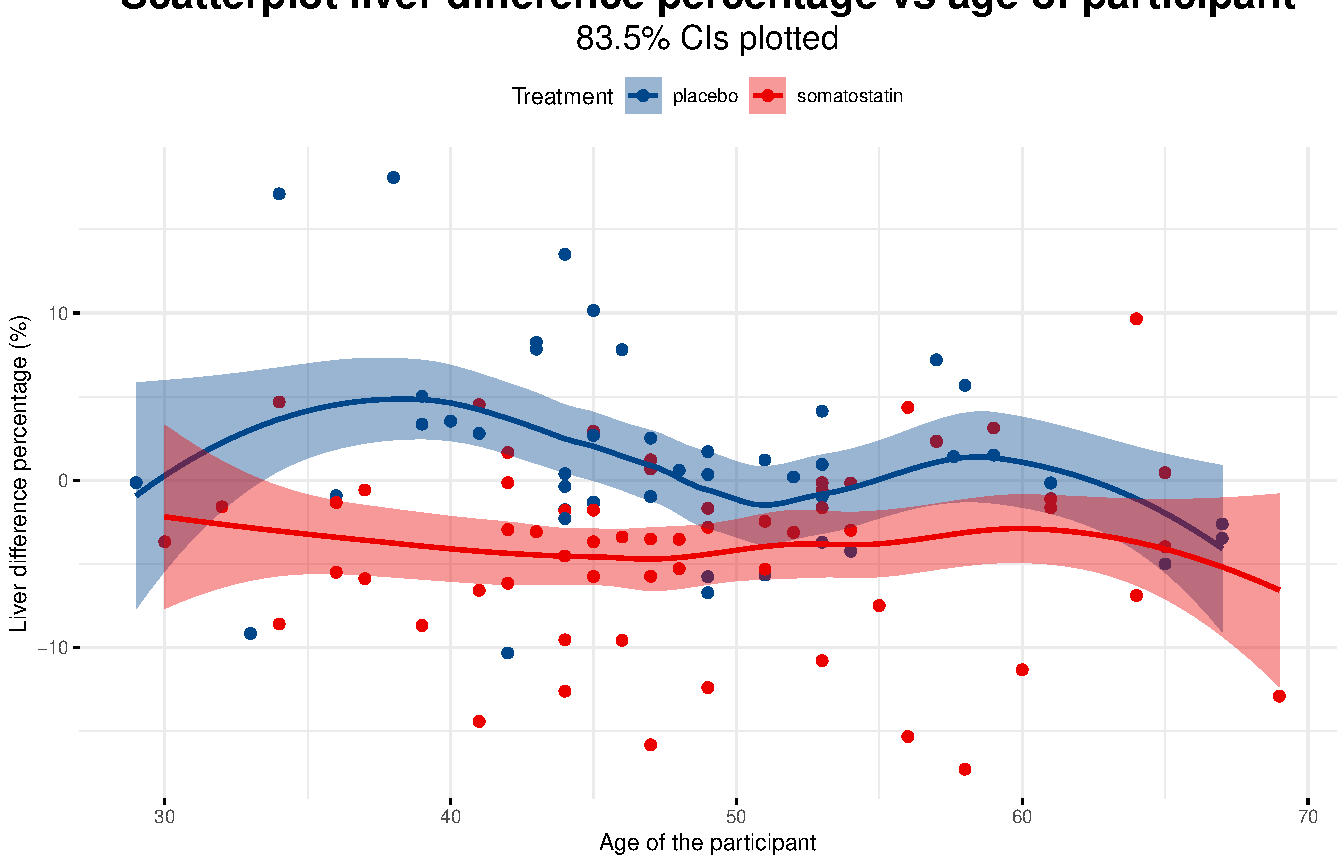
\includegraphics{Figs/unnamed-chunk-5-1.pdf}
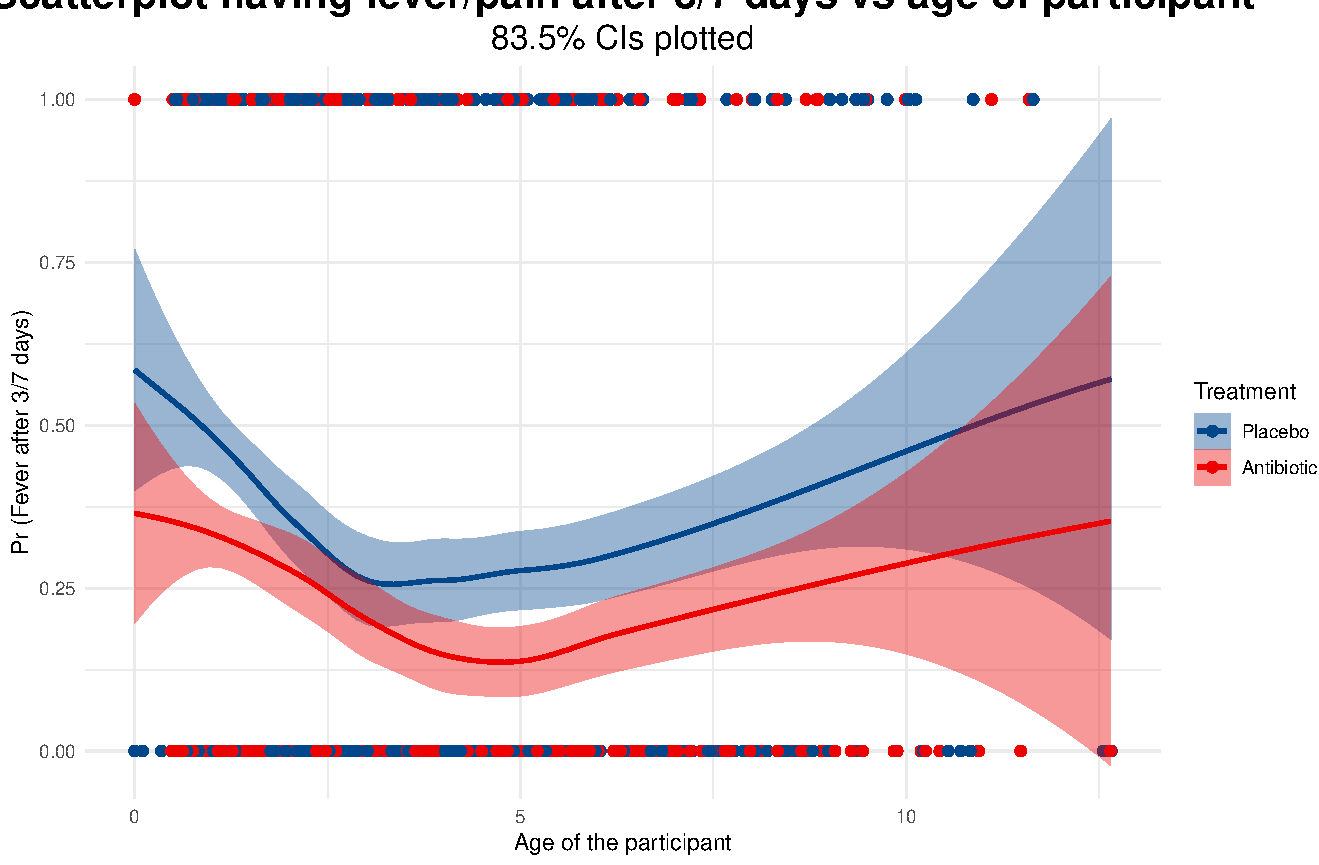
\includegraphics{Figs/unnamed-chunk-5-2.pdf}
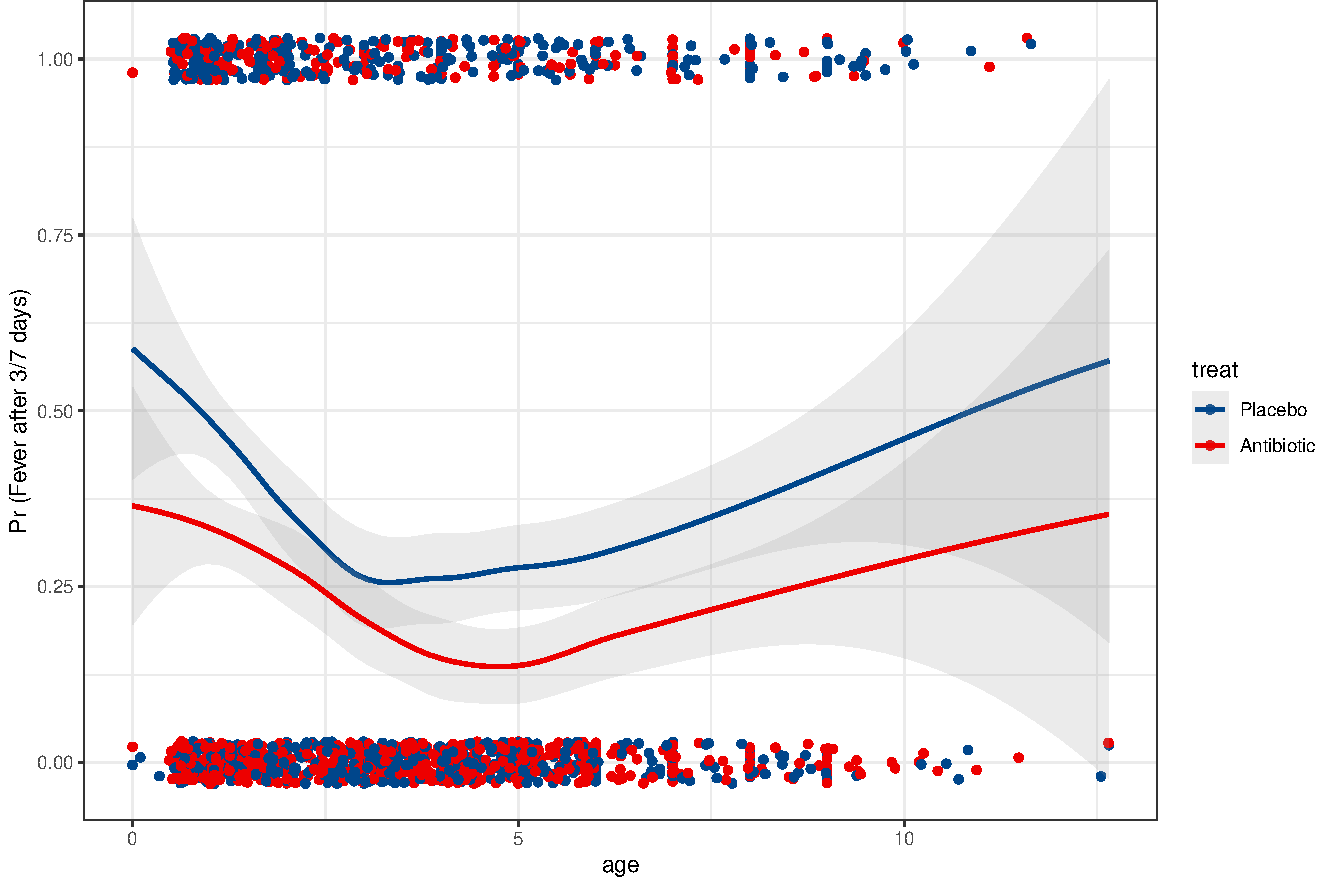
\includegraphics{Figs/unnamed-chunk-5-3.pdf}

We can see a linear association in the liver data set, while in the
acute otitis media data set a quadratic.

\hypertarget{two-stage-smoothing-splines}{%
\subsection{Two-stage smoothing
splines}\label{two-stage-smoothing-splines}}

In the acute otitis media data-set we had convergence problems and some
results were unrealistic\ldots{} \emph{Interactions are problematic.
This approach is difficult and needs more attention}.

\hypertarget{one-stage-smoothing-splines}{%
\subsection{One-stage smoothing
splines}\label{one-stage-smoothing-splines}}

In contrast with linear regression models, in smoothing spline models we
cannot directly interpret the shape of the regression line from the
summary estimates describing the spline function. Therefore,
visualization is an important tool to investigate effect modification.
We show that women younger than 57 have a treatment benefit, probably
due to menopause.

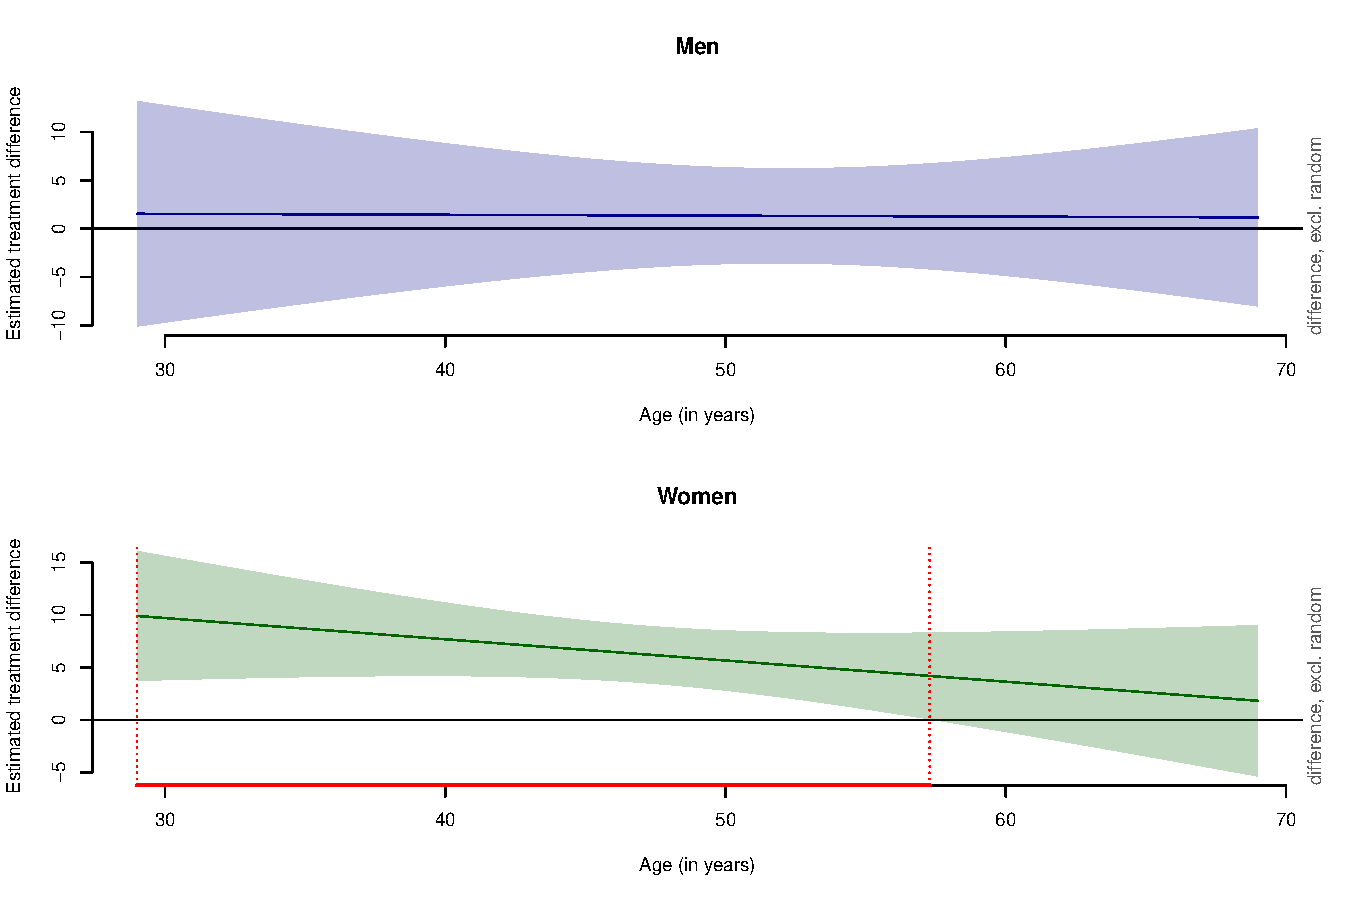
\includegraphics{Figs/One-Stage smoothing splines in Somatostatin-1.pdf}

\hypertarget{two-stage-fractional-polynomials}{%
\subsection{Two-stage Fractional
Polynomials}\label{two-stage-fractional-polynomials}}

\emph{Overall FP, where the FSP is applied in the pooled data, in order
to find the best FP (stratified by data-set).}

We extracted the fractional polynomial transformations for age per
treatment group and stratified per Study. Then we fit a GLM per trial
with this overall FP. The FP for the somatostatin data was linear. In
this method we couldn't investigate three-way interactions, as 2 studies
had insufficient \textbf{female} participants and limited sample size.

\begin{table}[H]
\centering
\resizebox{\linewidth}{!}{
\begin{tabular}{>{\bfseries\raggedright\arraybackslash}p{10em}>{\raggedleft\arraybackslash}p{10em}>{\raggedleft\arraybackslash}p{6em}>{\raggedleft\arraybackslash}p{10em}rrr}
\toprule
  & Estimate & Std. Error & z & Pr(>|z|) & 95\%ci.lb & 95\%ci.ub\\
\midrule
\rowcolor{gray!6}  Intercept & -0.7000481 & 0.2768177 & -2.5289135 & 0.0114416 & -1.2426008 & -0.1574953\\
Treatment & -0.3626153 & 0.1761254 & -2.0588473 & 0.0395089 & -0.7078148 & -0.0174159\\
\rowcolor{gray!6}  FP(Age) & -0.1023500 & 0.6301791 & -0.1624142 & 0.8709797 & -1.3374783 & 1.1327783\\
Bilateral & 0.1705120 & 0.3354571 & 0.5082976 & 0.6112446 & -0.4869718 & 0.8279959\\
\rowcolor{gray!6}  Treatment x FP(Age) & -0.6514992 & 0.9316185 & -0.6993197 & 0.4843523 & -2.4774380 & 1.1744396\\
\addlinespace
Treatment x Bilateral & -0.3189915 & 0.3332131 & -0.9573197 & 0.3384059 & -0.9720772 & 0.3340942\\
\rowcolor{gray!6}  Treatment x FP(Age) & -3.3502458 & 1.4964578 & -2.2387839 & 0.0251700 & -6.2832493 & -0.4172423\\
Treatment x FP(Age) x Bilateral & 0.9885212 & 2.1710792 & 0.4553133 & 0.6488839 & -3.2667158 & 5.2437582\\
\bottomrule
\end{tabular}}
\end{table}

\begin{table}[t]

\caption{\label{tab:MFP algorithm for AOM}Chi-squared test:}
\centering
\begin{tabular}{rrr}
\toprule
chi2 & df & P\\
\midrule
8.251 & 3 & 0.041\\
\bottomrule
\end{tabular}
\end{table}

We couldn't show that age is an effect modifier on 0.05 \(\alpha\)
significance level.

\hypertarget{study-wise-fp2-the-best-fp2-is-selected-for-each-study}{%
\subsection{Study-wise FP2, the best FP2 is selected for each
study}\label{study-wise-fp2-the-best-fp2-is-selected-for-each-study}}

The best fitting FP2s for the somatostatin per trial suffered from the
same problems as the overall FP.

Only 2 studies (Damoiseaux, Burke) could converge using the FP2 method.

\emph{Study wise selected FP, where the best fitting FP is extracted per
study}

The best fitting FPs for the somatostatin per trial were linear, so the
analysis is identical with the two-stage global polynomial.

\emph{Two-stage Global polynomials (coefficient pooling)}

For the Gevers et al.~data-analysis, we assumed a linear functional
form, as we had limited data (108 observations) and spending
\(2 \times p\) (degree of polynomial) \(\times J\) (trial number) was
considered inefficient. Furthermore, the initial pooled plot showed no
significant non-linearity. In contrast, for the Rovers et al.~we
observed an overall quadratic shape. Damoiseaux et al.~had age rounded
and the participants were only 1- and 2-years old children. To avoid
non-convergence of the log-binomial models we created a slight
artificial deviation for the Damoiseaux et al.~using the
\textbf{jitter()} command.

\begin{table}[H]
\centering
\resizebox{\linewidth}{!}{
\begin{tabular}{>{\bfseries\raggedright\arraybackslash}p{10em}>{\raggedleft\arraybackslash}p{10em}>{\raggedleft\arraybackslash}p{6em}>{\raggedleft\arraybackslash}p{10em}rrr}
\toprule
  & Estimate & Std. Error & z & Pr(>|z|) & 95\%ci.lb & 95\%ci.ub\\
\midrule
\rowcolor{gray!6}  intercept & -24.5770779 & 35.6471861 & -0.6894535 & 0.4905379 & -94.4442787 & 45.2901229\\
Treatment & -10.3277776 & 4.6129389 & -2.2388715 & 0.0251643 & -19.3689718 & -1.2865835\\
\rowcolor{gray!6}  Age & 0.9553693 & 1.1739279 & 0.8138228 & 0.4157465 & -1.3454872 & 3.2562258\\
Gender & 28.1468488 & 24.1964766 & 1.1632623 & 0.2447231 & -19.2773738 & 75.5710714\\
\rowcolor{gray!6}  Treatment x Age & 0.0917836 & 0.1060883 & 0.8651628 & 0.3869494 & -0.1161456 & 0.2997129\\
\addlinespace
Treatment x Gender & 4.0443188 & 2.0138605 & 2.0082417 & 0.0446176 & 0.0972247 & 7.9914129\\
\rowcolor{gray!6}  Age x Gender & -1.0078970 & 0.9465039 & -1.0648631 & 0.2869379 & -2.8630106 & 0.8472165\\
Treatment x Age x Gender & 0.0921206 & 0.1794881 & 0.5132409 & 0.6077828 & -0.2596696 & 0.4439108\\
\bottomrule
\end{tabular}}
\end{table}

\begin{table}[t]

\caption{\label{tab:Gasparini approach with mvmeta  for somatostatin}Chi-squared test:}
\centering
\begin{tabular}{rrr}
\toprule
chi2 & df & P\\
\midrule
2.363 & 2 & 0.307\\
\bottomrule
\end{tabular}
\end{table}

For the liver data set the two-stage meta-analysis of interaction terms
showed no statistically significant results. The reason we the same as
in splines and FPs. The per trial

\begin{table}[H]
\centering
\resizebox{\linewidth}{!}{
\begin{tabular}{>{\bfseries\raggedright\arraybackslash}p{10em}>{\raggedleft\arraybackslash}p{10em}>{\raggedleft\arraybackslash}p{6em}>{\raggedleft\arraybackslash}p{10em}rrrrr}
\toprule
  & intercept & Treatment & Age & Gender & Treatment x Age & Treatment x Gender & Age x Gender & Treatment x Age x Gender\\
\midrule
\rowcolor{gray!6}  Caroli & -100.326789 & -5.966345 & 3.4544383 & 78.757585 & -0.0343088 & 5.901427 & -3.0249067 & NA\\
Hogan & 22.297355 & -17.703486 & -0.4314088 & -8.238851 & 0.2164189 & 5.846667 & 0.1379887 & NA\\
\rowcolor{gray!6}  Keimpema & 9.099893 & -16.702593 & -0.1483457 & -5.421679 & 0.2485994 & 66.088189 & 0.0766080 & -1.238431\\
\bottomrule
\end{tabular}}
\end{table}

coefficients Little et al had no bilateral information. The study was
dropped.

\begin{table}[H]
\centering
\resizebox{\linewidth}{!}{
\begin{tabular}{>{\bfseries\raggedright\arraybackslash}p{10em}>{\raggedleft\arraybackslash}p{10em}>{\raggedleft\arraybackslash}p{6em}>{\raggedleft\arraybackslash}p{10em}rrr}
\toprule
  & Estimate & Std. Error & z & Pr(>|z|) & 95\%ci.lb & 95\%ci.ub\\
\midrule
\rowcolor{gray!6}  Intercept & 0.0631069 & 0.2830602 & 0.2229451 & 0.8235782 & -0.4916809 & 0.6178947\\
Treatment & 0.0963256 & 0.4175512 & 0.2306918 & 0.8175542 & -0.7220596 & 0.9147109\\
\rowcolor{gray!6}  Age & -0.4628134 & 0.1396732 & -3.3135444 & 0.0009212 & -0.7365679 & -0.1890589\\
Bilateral & 0.5839760 & 0.4490049 & 1.3006005 & 0.1933952 & -0.2960574 & 1.4640095\\
\rowcolor{gray!6}  Age\textasciicircum{}2 & 0.0426707 & 0.0142234 & 3.0000380 & 0.0026995 & 0.0147934 & 0.0705481\\
\addlinespace
Treatment x Age & -0.2703398 & 0.2198520 & -1.2296447 & 0.2188302 & -0.7012418 & 0.1605622\\
\rowcolor{gray!6}  Treatment x Bilateral & -1.6948939 & 0.7209635 & -2.3508733 & 0.0187294 & -3.1079564 & -0.2818313\\
Age x Bilateral & -0.0170794 & 0.3024478 & -0.0564707 & 0.9549669 & -0.6098663 & 0.5757075\\
\rowcolor{gray!6}  Treatment x Age\textasciicircum{}2 & 0.0309427 & 0.0233077 & 1.3275697 & 0.1843203 & -0.0147397 & 0.0766250\\
Age\textasciicircum{}2 x Bilateral & -0.0029376 & 0.0381286 & -0.0770444 & 0.9385882 & -0.0776684 & 0.0717932\\
\addlinespace
\rowcolor{gray!6}  Treatment x Age x Bilateral & 0.9218101 & 0.5367174 & 1.7174961 & 0.0858886 & -0.1301367 & 1.9737570\\
Treatment x Age\textasciicircum{}2 x Bilateral & -0.1106778 & 0.0768428 & -1.4403141 & 0.1497786 & -0.2612869 & 0.0399314\\
\bottomrule
\end{tabular}}
\end{table}

\begin{table}[t]

\caption{\label{tab:Gasparini approach with mvmeta  for AOM}Chi-squared test:}
\centering
\begin{tabular}{rrr}
\toprule
chi2 & df & P\\
\midrule
3.993 & 4 & 0.407\\
\bottomrule
\end{tabular}
\end{table}

\emph{One-stage IPD-MA}

\hypertarget{glmm-trees}{%
\subsection{GLMM-Trees}\label{glmm-trees}}

In the Gevers et al.~data-set we increased the level of significance
into \(\alpha\) =0.3, due to small sample size per trial.

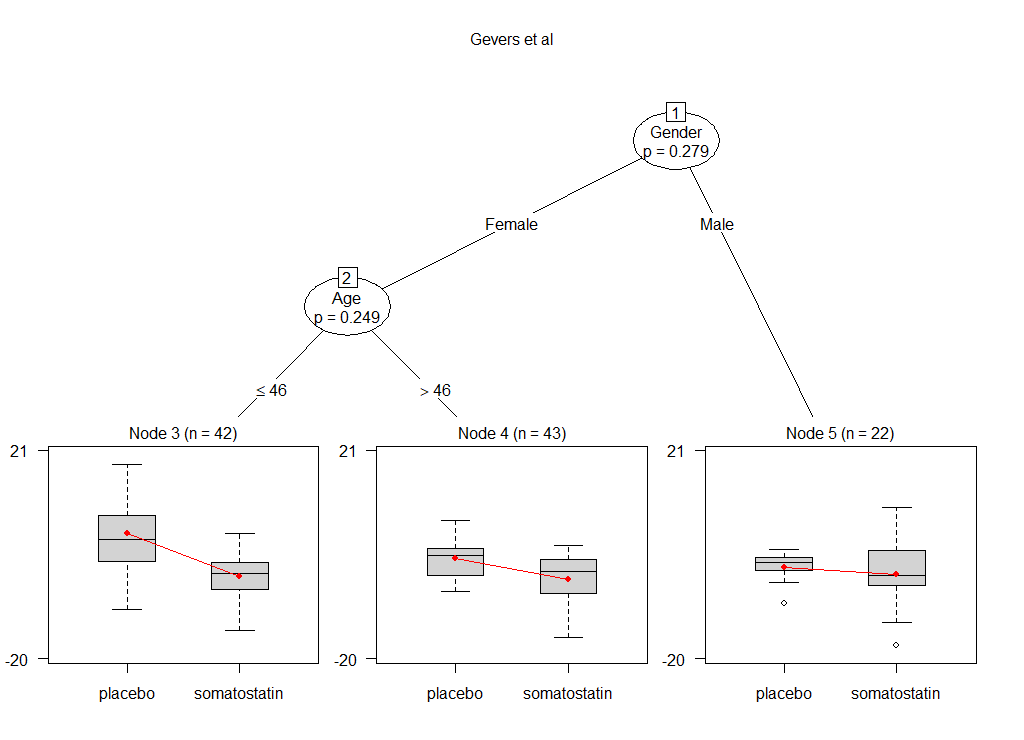
\includegraphics[width=0.8\linewidth,height=0.8\textheight]{Figs/SomatostatinTree}

\textbf{Figure.1 GLMM-tree for the liver data set}

We show that there is a difference between the treatment effects of
males and females. Furthermore, age seems to be an effect modifier in
the subgroup of females (cut-point at 46 years).

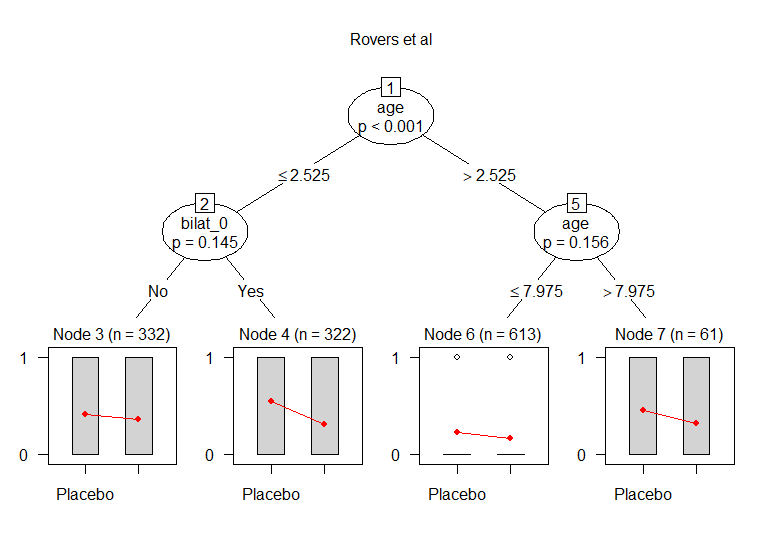
\includegraphics[width=0.8\linewidth,height=0.8\textheight]{Figs/AOMTree}

\textbf{Figure.2 GLMM-tree for the acute otitis media data set}

On the Rovers et al., dataset we show that age is a potential effect
modifier and we may also have a three-way interaction with bilateral
otitis.

\newpage

\hypertarget{section-2}{%
\subparagraph{}\label{section-2}}

\hypertarget{discussion}{%
\section{Discussion}\label{discussion}}

In our paper, we described and illustrated a variety of approaches to
explore, confirm, model or investigate for effect modification by a
continuous variable. Since clinical decision making often needs to
consider treatment effect in terms of available infrastructure, costs,
ethical constraints and other issues, it is important to assess how
treatment effect varies across relevant patient characteristics (rather
than merely establishing it does vary, as is commonly done in subgroup
analysis). Policy makers can then integrate all relevant evidence (such
as costs) to assess which cut-points should be recommended for decision
making. Our results showed that it is important to account for the
outcome-variable functional shape. Furthermore, we showed that
GLMM-trees can be a valuable exploratory tool to detect a potential
higher-level interaction. Also, two-stage methods suffered from trial
drop-outs and non-convergence, when trials with few participants were
analysed.

\hypertarget{comparison-with-literature}{%
\subsection{5.1 Comparison with
literature}\label{comparison-with-literature}}

Help needed

\hypertarget{strengths-and-limitations}{%
\subsection{5.2 Strengths and
limitations}\label{strengths-and-limitations}}

The major strength of our paper is the variety of approaches we
illustrated. In particular, we beside generalised linear mixed effects
models we also described and illustrated one and two-stage generalised
additive models using splines, two-stage fractional polynomials and we
proposed a one-stage fractional polynomial approach using a similar
intuitive method as Royston et al.~To our knowledge this the first study
describing and illustrating in empirical data sets the approaches
mentioned above. Furthermore, we also wish to point out some
limitations. I am writing them in bullets so that we extend them and
order them and write more:

\begin{itemize}
\item
  GAM approach identifies the point where
  E(\(\hat Y_{treated} - \hat Y_{control} \pm 1.96 \times SE_{diff}\) )
  crosses 0. This measure can be further developed (ideas are welcome)
  for example, the percentage of the wrongly treated (Joanna's idea),
  posterior confidence bands (Bayesian approach)
\item
  Our data were limited in linear and quadratic shapes
\item
  Liver data set had small trials and didn't converge (in two-stage
  approach)
\item
  GAMs have a lot of variations nevertheless, we used the most
  reasonable
\item
  No simulation so we don't really know the truth
\end{itemize}

\hypertarget{implications-for-practice}{%
\subsection{5.3 Implications for
practice}\label{implications-for-practice}}

\hypertarget{conclusions}{%
\subsection{5.4 Conclusions}\label{conclusions}}

We propose the use of one-stage generalised additive model with
smoothing spline. This approach makes no assumptions over the functional
shape and the cut-point where it changes, as its primary goal is to
estimate them both. Furthermore, combined with the treatment effect plot
we can easily identify the point where the treatment effect is altered,
(equivalent to the CIs of the RD).

\newpage

\hypertarget{section-3}{%
\subparagraph{}\label{section-3}}

\hypertarget{references}{%
\section*{References}\label{references}}
\addcontentsline{toc}{section}{References}

\hypertarget{refs}{}
\leavevmode\hypertarget{ref-Debray_2015}{}%
{[}1{]} Debray TPA, Moons KGM, Valkenhoef G van, Efthimiou O, Hummel N,
Groenwold RHH, et al. Get real in individual participant data (IPD)
meta-analysis: A review of the methodology. Research Synthesis Methods
2015;6:293--309.
doi:\href{https://doi.org/10.1002/jrsm.1160}{10.1002/jrsm.1160}.

\leavevmode\hypertarget{ref-Maroeska_2012}{}%
{[}2{]} Rovers M, Reitsma JB. {[}The meta-analysis of data from
individual patients{]}. Nederlands Tijdschrift Voor Geneeskunde
2012;156:A4743.

\leavevmode\hypertarget{ref-Tierney_2015}{}%
{[}3{]} Tierney JF, Vale C, Riley R, Smith CT, Stewart L, Clarke M, et
al. Individual participant data (IPD) meta-analyses of randomised
controlled trials: Guidance on their use. PLOS Medicine
2015;12:e1001855.
doi:\href{https://doi.org/10.1371/journal.pmed.1001855}{10.1371/journal.pmed.1001855}.

\leavevmode\hypertarget{ref-Royston_2005}{}%
{[}4{]} Royston P, Altman DG, Sauerbrei W. Dichotomizing continuous
predictors in multiple regression: A bad idea. Statistics in Medicine
2005;25:127--41.
doi:\href{https://doi.org/10.1002/sim.2331}{10.1002/sim.2331}.

\leavevmode\hypertarget{ref-Altman_2006}{}%
{[}5{]} Altman DG. The cost of dichotomising continuous variables. BMJ
2006;332:1080--0.
doi:\href{https://doi.org/10.1136/bmj.332.7549.1080}{10.1136/bmj.332.7549.1080}.

\leavevmode\hypertarget{ref-Austin_2004}{}%
{[}6{]} Austin PC, Brunner LJ. Inflation of the type i error rate when a
continuous confounding variable is categorized in logistic regression
analyses. Statistics in Medicine 2004;23:1159--78.
doi:\href{https://doi.org/10.1002/sim.1687}{10.1002/sim.1687}.

\leavevmode\hypertarget{ref-Maxwell_1993}{}%
{[}7{]} Maxwell SE, Delaney HD. Bivariate median splits and spurious
statistical significance. Psychological Bulletin 1993;113:181--90.
doi:\href{https://doi.org/10.1037/0033-2909.113.1.181}{10.1037/0033-2909.113.1.181}.

\leavevmode\hypertarget{ref-Weinberg_1995}{}%
{[}8{]} Weinberg C. How bad is categorization? Epidemiology
1995;6:345--6.
doi:\href{https://doi.org/10.1097/00001648-199507000-00002}{10.1097/00001648-199507000-00002}.

\leavevmode\hypertarget{ref-J_rgensen_2016}{}%
{[}9{]} Jørgensen TSH, Osler M, Ängquist LH, Zimmermann E, Christensen
GT, Sørensen TIA. The u-shaped association of body mass index with
mortality: Influence of the traits height, intelligence, and education.
Obesity 2016;24:2240--7.
doi:\href{https://doi.org/10.1002/oby.21615}{10.1002/oby.21615}.

\leavevmode\hypertarget{ref-royston_interaction_2013}{}%
{[}10{]} Royston P, Sauerbrei W. Interaction of treatment with a
continuous variable: Simulation study of significance level for several
methods of analysis. Statistics in Medicine 2013;32:3788--803.
doi:\href{https://doi.org/10.1002/sim.5813}{10.1002/sim.5813}.

\leavevmode\hypertarget{ref-Sun_2010}{}%
{[}11{]} Sun X, Briel M, Walter SD, Guyatt GH. Is a subgroup effect
believable? Updating criteria to evaluate the credibility of subgroup
analyses. BMJ 2010;340:c117--7.
doi:\href{https://doi.org/10.1136/bmj.c117}{10.1136/bmj.c117}.

\leavevmode\hypertarget{ref-Sauerbrei_2011}{}%
{[}12{]} Sauerbrei W, Royston P. A new strategy for meta-analysis of
continuous covariates in observational studies. Statistics in Medicine
2011;30:3341--60.
doi:\href{https://doi.org/10.1002/sim.4333}{10.1002/sim.4333}.

\leavevmode\hypertarget{ref-Legha_2018}{}%
{[}13{]} Legha A, Riley RD, Ensor J, Snell KIE, Morris TP, Burke DL.
Individual participant data meta-analysis of continuous outcomes: A
comparison of approaches for specifying and estimating one-stage models.
Statistics in Medicine n.d.
doi:\href{https://doi.org/10.1002/sim.7930}{10.1002/sim.7930}.

\leavevmode\hypertarget{ref-Wang_2016}{}%
{[}14{]} Wang XV, Cole B, Bonetti M, Gelber RD. Meta-STEPP:
Subpopulation treatment effect pattern plot for individual patient data
meta-analysis. Statistics in Medicine 2016;35:3704--16.
doi:\href{https://doi.org/10.1002/sim.6958}{10.1002/sim.6958}.

\leavevmode\hypertarget{ref-Rovers_2006}{}%
{[}15{]} Rovers MM, Glasziou P, Appelman CL, Burke P, McCormick DP,
Damoiseaux RA, et al. Antibiotics for acute otitis media: A
meta-analysis with individual patient data. The Lancet
2006;368:1429--35.
doi:\href{https://doi.org/10.1016/s0140-6736(06)69606-2}{10.1016/s0140-6736(06)69606-2}.

\leavevmode\hypertarget{ref-Gevers_2013}{}%
{[}16{]} Gevers TJG, Inthout J, Caroli A, Ruggenenti P, Hogan MC, Torres
VE, et al. Young women with polycystic liver disease respond best to
somatostatin analogues: A pooled analysis of individual patient data.
Gastroenterology 2013;145:357--365.e2.
doi:\href{https://doi.org/10.1053/j.gastro.2013.04.055}{10.1053/j.gastro.2013.04.055}.

\leavevmode\hypertarget{ref-Breiman_2017}{}%
{[}17{]} Breiman L. Classification and regression trees. Routledge;
2017.
doi:\href{https://doi.org/10.1201/9781315139470}{10.1201/9781315139470}.

\leavevmode\hypertarget{ref-Zeileis_2008}{}%
{[}18{]} Zeileis A, Hothorn T, Hornik K. Model-based recursive
partitioning. Journal of Computational and Graphical Statistics
2008;17:492--514.
doi:\href{https://doi.org/10.1198/106186008x319331}{10.1198/106186008x319331}.

\leavevmode\hypertarget{ref-Su_2009}{}%
{[}19{]} Su X, Tsai C-L, Wang H, Nickerson DM, Li B. Subgroup analysis
via recursive partitioning. SSRN Electronic Journal 2009.
doi:\href{https://doi.org/10.2139/ssrn.1341380}{10.2139/ssrn.1341380}.

\leavevmode\hypertarget{ref-Fokkema_2017}{}%
{[}20{]} Fokkema M, Smits N, Zeileis A, Hothorn T, Kelderman H.
Detecting treatment-subgroup interactions in clustered data with
generalized linear mixed-effects model trees. Behavior Research Methods
2017.
doi:\href{https://doi.org/10.3758/s13428-017-0971-x}{10.3758/s13428-017-0971-x}.

\leavevmode\hypertarget{ref-Abo_Zaid_2013}{}%
{[}21{]} Abo-Zaid G, Guo B, Deeks JJ, Debray TPA, Steyerberg EW, Moons
KGM, et al. Individual participant data meta-analyses should not ignore
clustering. Journal of Clinical Epidemiology 2013;66:865--873.e4.
doi:\href{https://doi.org/10.1016/j.jclinepi.2012.12.017}{10.1016/j.jclinepi.2012.12.017}.

\leavevmode\hypertarget{ref-Royston_1994}{}%
{[}22{]} Royston P, Altman DG. Regression using fractional polynomials
of continuous covariates: Parsimonious parametric modelling. Applied
Statistics 1994;43:429.
doi:\href{https://doi.org/10.2307/2986270}{10.2307/2986270}.

\leavevmode\hypertarget{ref-Ambler_2001}{}%
{[}23{]} Ambler G, Royston P. Fractional polynomial model selection
procedures: Investigation of type i error rate. Journal of Statistical
Computation and Simulation 2001;69:89--108.
doi:\href{https://doi.org/10.1080/00949650108812083}{10.1080/00949650108812083}.

\leavevmode\hypertarget{ref-Sauerbrei_1999}{}%
{[}24{]} Sauerbrei W, Royston P. Building multivariable prognostic and
diagnostic models: Transformation of the predictors by using fractional
polynomials. Journal of the Royal Statistical Society: Series A
(Statistics in Society) 1999;162:71--94.
doi:\href{https://doi.org/10.1111/1467-985x.00122}{10.1111/1467-985x.00122}.

\leavevmode\hypertarget{ref-White_2018}{}%
{[}25{]} White IR, Kaptoge S, Royston P, and WS. Meta-analysis of
non-linear exposure-outcome relationships using individual participant
data: A comparison of two methods. Statistics in Medicine 2018.
doi:\href{https://doi.org/10.1002/sim.7974}{10.1002/sim.7974}.

\leavevmode\hypertarget{ref-McCullagh_1983}{}%
{[}26{]} McCullagh P, Nelder JA. An outline of generalized linear
models. In:. Generalized linear models, Springer US; 1983, pp. 15--34.
doi:\href{https://doi.org/10.1007/978-1-4899-3244-0_2}{10.1007/978-1-4899-3244-0\_2}.

\leavevmode\hypertarget{ref-Long_2010}{}%
{[}27{]} Long J, Ryoo J. Using fractional polynomials to model
non-linear trends in longitudinal data. British Journal of Mathematical
and Statistical Psychology 2010;63:177--203.
doi:\href{https://doi.org/10.1348/000711009x431509}{10.1348/000711009x431509}.

\leavevmode\hypertarget{ref-Johnson_2012}{}%
{[}28{]} Johnson W, Balakrishna N, Griffiths PL. Modeling physical
growth using mixed effects models. American Journal of Physical
Anthropology 2012;150:58--67.
doi:\href{https://doi.org/10.1002/ajpa.22128}{10.1002/ajpa.22128}.

\leavevmode\hypertarget{ref-Akaike_1974}{}%
{[}29{]} Akaike H. A new look at the statistical model identification.
In:. Springer series in statistics, Springer New York; 1974, pp.
215--22.
doi:\href{https://doi.org/10.1007/978-1-4612-1694-0_16}{10.1007/978-1-4612-1694-0\_16}.

\leavevmode\hypertarget{ref-Schwarz_1978}{}%
{[}30{]} Schwarz G. Estimating the dimension of a model. The Annals of
Statistics 1978;6:461--4.
doi:\href{https://doi.org/10.1214/aos/1176344136}{10.1214/aos/1176344136}.

\leavevmode\hypertarget{ref-Hua_2016}{}%
{[}31{]} Hua H, Burke DL, Crowther MJ, Ensor J, Smith CT, Riley RD.
One-stage individual participant data meta-analysis models: Estimation
of treatment-covariate interactions must avoid ecological bias by
separating out within-trial and across-trial information. Statistics in
Medicine 2016;36:772--89.
doi:\href{https://doi.org/10.1002/sim.7171}{10.1002/sim.7171}.


\end{document}
